\chapter{Production Refined Fracture Validation and Convergence}
\label{chap:production_refined_validation}

This chapter documents the systematic verification, mesh adequacy, and multifaceted numerical convergence of the Mode-I crack propagation problem under the qualified 3-layer UEL phase-field finite element implementation. In accordance with thesis objectives, convergence is evaluated across spatial discretization, temporal time incrementation, physical length-scale regularization, and global energetic balance.

\section{Spatial Mesh Resolution Series ($S_1$--$S_4$)}
\label{sec:spatial_series_study}

A spatial discretization sweep was conducted across four uniform quad-dominant finite element meshes spanning element edge lengths from $h = 3.0\,\mu\text{m}$ ($S_1$, $15{,}192$ elements) down to $h = 1.25\,\mu\text{m}$ ($S_4$, $51{,}408$ elements), holding the physical regularisation length scale strictly constant at $l_0 = 7.5\,\mu\text{m}$ ($h/l_0 \in [0.167, 0.400]$). A historical fine-mesh result ($h = 1.0\,\mu\text{m}$, $69{,}384$ elements, Job \texttt{1406019.mmaster02}) was also analyzed:
\begin{enumerate}
    \item \textbf{Initial Elastic Stiffness $K_0$}: Evaluated over the linear elastic regime ($u \le 1.0\,\mu\text{m}$). $K_0$ varies by less than $0.09\%$ across all meshes ($137.945520\,\text{kN/mm}$ for $S_1$ to $137.823301\,\text{kN/mm}$ for $h=1.0\,\mu\text{m}$, $R^2 > 0.999999$), classified as \textbf{\texttt{CONVERGED / STABLE}} (Table~\ref{tab:spatial_series_thesis}, Figure~\ref{fig:spatial_convergence_thesis}).
    \item \textbf{Peak Reaction Force $F_{\max}$ and Displacement $u_{\mathrm{peak}}$}: Refinement systematically lowers the peak force from $0.7578\,\text{kN}$ ($S_1$) to $0.7255\,\text{kN}$ ($h=1.0\,\mu\text{m}$), a monotonic reduction of $4.26\%$. Concurrently, peak displacement advances from $5.857\,\mu\text{m}$ to $5.575\,\mu\text{m}$ (a $4.81\%$ shift), classified as \textbf{\texttt{MESH-SENSITIVE}}.
\end{enumerate}

\begin{table}[htbp]
\centering
\caption{Spatial mesh resolution convergence metrics at fixed $l_0 = 7.5\,\mu\text{m}$.}
\label{tab:spatial_series_thesis}
\small
\begin{tabular}{lrrrrrr}
\toprule
\textbf{Mesh ID} & $h$ [$\mu\text{m}$] & $h/l_0$ & \textbf{Elements} & $K_0$ [kN/mm] & $F_{\max}$ [kN] & $u_{\mathrm{peak}}$ [$\mu\text{m}$] \\
\midrule
$S_1$ (Baseline) & $3.00$ & $0.400$ & $15{,}192$ & $137.945520$ & $0.757778$ & $5.857$ \\
$S_2$ & $2.00$ & $0.267$ & $32{,}130$ & $137.876115$ & $0.741210$ & $5.714$ \\
$S_3$ & $1.50$ & $0.200$ & $41{,}912$ & $137.857608$ & $0.732196$ & $5.633$ \\
$S_4$ & $1.25$ & $0.167$ & $51{,}408$ & $137.841200$ & $0.731180$ & $5.620$ \\
Historical Fine & $1.00$ & $0.133$ & $69{,}384$ & $137.823301$ & $0.725501$ & $5.575$ \\
\bottomrule
\end{tabular}
\end{table}

\begin{figure}[htbp]
\centering
\includegraphics[width=0.80\textwidth]{fig_mode1_spatial_fu_convergence.pdf}
\caption[Force-displacement curves across uniform mesh resolutions.]{Mode-I tensile force-displacement response across uniform mesh resolutions ($S_1$--$S_4$ and historical fine mesh), showing identical elastic stiffness and systematic peak load mesh sensitivity.}
\label{fig:spatial_convergence_thesis}
\end{figure}

\begin{figure}[htbp]
\centering
\includegraphics[width=0.90\textwidth]{fig_mode1_spatial_convergence_metrics.pdf}
\caption[Scaling metrics across spatial resolution sweep.]{Discretization ratio ($h/l_0$) scaling metrics: (a) initial stiffness $K_0$ invariance; (b) peak reaction force $F_{\max}$; (c) peak displacement $u_{\mathrm{peak}}$; (d) matched-displacement external work $W_{\mathrm{trap}}$ at $u = 5.50\,\mu\text{m}$.}
\label{fig:spatial_metrics_thesis}
\end{figure}

\section{Temporal Time-Increment Scaling ($T_1$--$T_3$)}
\label{sec:temporal_series_study}

Time incrementation was evaluated across three schedules on the baseline $S_1$ mesh: Case $T_1$ (coarse $2\times$, $3{,}500$ incs), Case $T_2$ (nominal $1\times$, $7{,}000$ incs), and Case $T_3$ (fine $0.5\times$, Job \texttt{1406317.mmaster02}, $10{,}022$ incs reaching $u = 10.0\,\mu\text{m}$):
\begin{itemize}
    \item \textbf{Peak Load Invariance}: Initial stiffness varies by $<0.001\%$, and peak reaction force varies by $<0.07\%$ ($0.75815 \to 0.75763\,\text{kN}$), establishing temporal convergence through the peak load (\textbf{\texttt{CONVERGED / STABLE}}, Figure~\ref{fig:temporal_convergence_thesis}).
    \item \textbf{Post-Peak Energy Sensitivity}: Terminal trapezoidal boundary work $W_{\mathrm{trap}}$ varies by $3.24\%$ ($2.41011 \to 2.33189\,\text{mJ}$), and normalized two-term bookkeeping discrepancy $\mathcal{R}_{\mathrm{bookkeeping}} = W_{\mathrm{trap}} - (E_{\mathrm{elas}} + E_{\mathrm{frac}})$ shifts from $+0.378\%$ to $+3.541\%$, classified as \textbf{\texttt{TEMPORALLY SENSITIVE}}.
\end{itemize}

\begin{figure}[htbp]
\centering
\includegraphics[width=0.78\textwidth]{fig_mode1_temporal_convergence.pdf}
\caption[Temporal convergence across time incrementation scales.]{Temporal convergence across time increment scales ($T_1$: $2\times$, $T_2$: $1\times$, $T_3$: $0.5\times$), demonstrating step-size invariance of the mechanical peak.}
\label{fig:temporal_convergence_thesis}
\end{figure}

\section{Adaptive Mesh Temporal Refinement Audit ($2\times$ Refinement)}
\label{sec:adaptive_temporal_refinement_audit_thesis}

To verify temporal convergence on the non-uniform error-indicator refined mesh, a controlled $2\times$ temporal refinement diagnostic (Job \texttt{1410027.mmaster02}, $8{,}958$ increments) was audited against the baseline canonical ET1 solve (Job \texttt{1409982.mmaster02}, $4{,}890$ increments) on the $14{,}483$-element discretization (Table~\ref{tab:adaptive_temporal_audit_thesis}, Figures~\ref{fig:adaptive_temporal_fu}--\ref{fig:adaptive_temporal_energy}).

\begin{table}[htbp]
\centering
\caption{Adaptive mesh $2\times$ temporal refinement audit metrics.}
\label{tab:adaptive_temporal_audit_thesis}
\small
\begin{tabular}{lrrr}
\toprule
\textbf{Metric} & \textbf{Baseline ($1.00\,\text{nm}$)} & \textbf{$2\times$ Refined ($0.50\,\text{nm}$)} & \textbf{Relative Difference} \\
\midrule
PBS Job ID & \texttt{1409982.mmaster02} & \texttt{1410027.mmaster02} & --- \\
Step 1 Displacement Step ($\Delta u_1$) & $2.50\,\text{nm}$ & $1.25\,\text{nm}$ & $-50.0\%$ \\
Step 2 Displacement Step ($\Delta u_2$) & $1.00\,\text{nm}$ & $0.50\,\text{nm}$ & $-50.0\%$ \\
Completed Increments & $4{,}890$ & $8{,}958$ & $+83.2\%$ \\
Elastic Stiffness $K_0$ & $137.909558\,\text{kN/mm}$ & $137.909975\,\text{kN/mm}$ & $\mathbf{+0.000302\%}$ \\
Peak Force $F_{\max}$ & $0.743701\,\text{kN}$ & $0.743530\,\text{kN}$ & $\mathbf{-0.0229\%}$ \\
Displacement at Peak $u_{\mathrm{peak}}$ & $5.733\,\mu\text{m}$ & $5.730\,\mu\text{m}$ & $\mathbf{-0.052\%}$ \\
Peak Model Energy $E_{\mathrm{model}}(u_{\mathrm{peak}})$ & $2.205225\,\text{mJ}$ & $2.205225\,\text{mJ}$ & $\mathbf{0.000000\%}$ \\
Maximum Pre-Peak $|\Delta F|/F$ & --- & --- & $\le 0.0436\%$ \\
Reached Common Displacement & \multicolumn{2}{c}{$u \in [0.0, 7.46970\,\mu\text{m}]$} & Common domain \\
Governing Pre-Peak Classification & \multicolumn{3}{c}{\textbf{\texttt{QUALIFIED\_OVER\_PREPEAK\_INTERVAL\_ONLY (TEMPORALLY\_STABLE)}}} \\
Governing Post-Peak Classification & \multicolumn{3}{c}{\textbf{\texttt{TEMPORALLY\_SENSITIVE\_POSTPEAK}}} \\
\bottomrule
\end{tabular}
\end{table}

\begin{figure}[htbp]
\centering
\includegraphics[width=0.82\textwidth]{fig_mode1_stage14_temporal_convergence_fu.pdf}
\caption[Adaptive mesh force-displacement comparison under $2\times$ temporal refinement.]{Adaptive mesh force--displacement comparison between baseline ($1.00\,\text{nm}$) and $2\times$ refined ($0.50\,\text{nm}$) step size on the $14{,}483$-element discretization, demonstrating strict pre-peak coincidence and post-peak cutback bifurcation.}
\label{fig:adaptive_temporal_fu}
\end{figure}

\begin{figure}[htbp]
\centering
\includegraphics[width=0.82\textwidth]{fig_mode1_stage14_temporal_discrepancy.pdf}
\caption[Pointwise reaction force discrepancy across displacement history.]{Pointwise reaction force discrepancy $\Delta F = F_{2\times} - F_{\mathrm{base}}$ and relative error $|\Delta F|/F$, confirming sub-$0.044\%$ discrepancy throughout the pre-peak regime.}
\label{fig:adaptive_temporal_discrepancy}
\end{figure}

\begin{figure}[htbp]
\centering
\includegraphics[width=0.82\textwidth]{fig_mode1_stage14_temporal_energy_evolution.pdf}
\caption[Global energetic evolution under temporal refinement.]{Evolution of elastic strain energy $E_{\mathrm{elas}}$, fracture surface energy $E_{\mathrm{frac}}$, and external work $W_{\mathrm{trap}}$ on the adaptive mesh, showing exact pre-peak parity.}
\label{fig:adaptive_temporal_energy}
\end{figure}

\subsection{Post-Peak Wake Cutback Exhaustion Mechanism}
In the post-peak softening regime, both models track identical softening slopes through $u \approx 7.0\,\mu\text{m}$. Beyond $u = 7.0\,\mu\text{m}$, the crack tip propagates past $x = 0.55\,\text{mm}$, leaving a fully severed wake ($d \approx 0.999$, $\sigma \approx 0$). In this severed wake, residual phase-field corrections ($c_{\max} \approx 2.6\times 10^{-6}$) interact with Abaqus standard convergence controls:
\begin{equation}
\label{eq:abaqus_cn_check}
c_{\max} \le C_n\,\Delta u_{\mathrm{inc}}.
\end{equation}
Because the $2\times$ refined model imposes $\Delta u_{\mathrm{inc}} = 0.50\,\text{nm}$ (halved relative to baseline $\Delta u_{\mathrm{inc}} = 1.00\,\text{nm}$), the dimensional tolerance threshold $C_n \Delta u_{\mathrm{inc}}$ is strictly $2\times$ tighter. Consequently, minute mathematical corrections in stress-free, fully broken elements exceed the tighter tolerance, triggering successive solver cutbacks until minimum time increment exhaustion occurs at $u = 7.470\,\mu\text{m}$ ($8{,}958$ increments) in the refined case, compared to $u = 7.889\,\mu\text{m}$ ($4{,}890$ increments) in the baseline.

To rule out user subroutine implementation defects, numerical tangent Jacobian consistency was evaluated to machine precision ($\max |\Delta| = 1.36\times 10^{-14}$), confirming exact analytical Jacobian symmetry and consistency. The post-peak cutback is thus established as a solver convergence-normalization artifact:
\begin{center}
  \textbf{\texttt{POST\_FRACTURE\_CONVERGENCE\_NORMALIZATION\_SENSITIVITY\_VERIFIED}}
\end{center}
which governs the active diagnostic investigation (Job \texttt{1410180.mmaster02}, testing $C_n = 0.50$ relaxation).

\section{Adaptive Remeshing Spatial Series ($A_1$--$A_4$)}
\label{sec:adaptive_series_study}

Across adaptive cases $A_1$--$A_4$ (Figure~\ref{fig:adaptive_thesis}), all meshes reproduce the reference elastic stiffness $K_0 \approx 137.85\,\text{kN/mm}$ within $0.09\%$. In the post-peak softening regime, coarser background meshes ($A_2$--$A_4$) sustain elevated residual resistance, classified as \textbf{\texttt{OBSERVED\_FORCE\_PLATEAU (CRACK-PINNING HYPOTHESIS / NOT YET INDEPENDENTLY PROVEN)}}.

\begin{figure}[htbp]
\centering
\includegraphics[width=0.78\textwidth]{fig_mode1_adaptive_convergence.pdf}
\caption[Force-displacement curves for native adaptive cases.]{Force-displacement curves for native adaptive cases ($A_1$--$A_4$) alongside baseline $S_1$.}
\label{fig:adaptive_thesis}
\end{figure}

\section{Three-Point Physical Length-Scale Study ($l_0$ on Fixed $S_3$ Mesh)}
\label{sec:length_scale_study}

A controlled physical length-scale sensitivity study was audited on the fixed $S_3$ mesh ($41{,}912$ continuum finite elements, $42{,}491$ FE mesh nodes, $42{,}492$ total input nodes with RP \texttt{999999}) across three regularization lengths $l_0 \in \{7.5, 11.25, 15.0\}\,\mu\text{m}$ (Table~\ref{tab:l0_study_thesis}, Figures~\ref{fig:clean_l0_fu_thesis} and \ref{fig:clean_l0_scaling_thesis}). Bitwise provenance audit confirms 100\% identical node coordinate hashes (\texttt{7599c30f...}) and element connectivity hashes (\texttt{96d085b2...}) across all three input decks, verifying a genuine single-variable physical study:
\begin{itemize}
    \item \textbf{Stiffness Invariance}: Initial structural stiffness $K_0$ varies from $137.857608$ to $137.676175\,\text{kN/mm}$ ($\Delta = 0.13\%$), classified as \textbf{\texttt{L0\_RESPONSE\_STABLE}}.
    \item \textbf{Peak Force and Displacement Sensitivity}: Peak reaction force drops monotonically from $0.732196\,\text{kN}$ ($l_0 = 7.5\,\mu\text{m}$) to $0.689540\,\text{kN}$ ($l_0 = 15.0\,\mu\text{m}$, a $5.83\%$ reduction), while displacement at peak shifts earlier from $5.633\,\mu\text{m}$ to $5.579\,\mu\text{m}$, classified as \textbf{\texttt{L0\_RESPONSE\_SENSITIVE}}.
    \item \textbf{Localization Bandwidth Scaling}: Transverse damage profile bandwidth $w_{0.5}$ scales linearly with $l_0$ ($w_{0.5} \approx 3.04\,l_0$: $20.79\,\mu\text{m} \to 34.41\,\mu\text{m} \to 45.44\,\mu\text{m}$), confirming theoretical gradient regularization.
    \item \textbf{Common Reached Domain \& Energy Status}: Analysis is strictly restricted to the common reached displacement domain $u \in [0.0, 5.839]\,\mu\text{m}$ with zero forward filling. Terminal energy comparison across the three cases is classified as \textbf{\texttt{ENERGY\_NOT\_YET\_QUALIFIED\_UNEQUAL\_ENDPOINTS\_AND\_PRE\_GATE6B\_SOURCE}}.
\end{itemize}

\begin{table}[htbp]
\centering
\caption{Three-point physical length-scale sensitivity metrics on fixed $S_3$ mesh ($41{,}912$ FE, $42{,}491$ FE nodes).}
\label{tab:l0_study_thesis}
\small
\begin{tabular}{lrrrrrrr}
\toprule
$l_0$ [$\mu\text{m}$] & \textbf{Job ID} & $\frac{h_{\min}}{l_0}$ & $K_0$ [kN/mm] & $F_{\max}$ [kN] & $u_{\mathrm{peak}}$ [$\mu\text{m}$] & $w_{0.5}$ [$\mu\text{m}$] & $\frac{w_{0.5}}{l_0}$ \\
\midrule
$7.50$ & \texttt{1406017.mmaster02} & $0.260$ & $137.857608$ & $0.732196$ & $5.633$ & $20.79$ & $2.77$ \\
$11.25$ & \texttt{1406895.mmaster02} & $0.174$ & $137.765563$ & $0.708402$ & $5.590$ & $34.41$ & $3.06$ \\
$15.00$ & \texttt{1406896.mmaster02} & $0.130$ & $137.676175$ & $0.689540$ & $5.579$ & $45.44$ & $3.03$ \\
\bottomrule
\end{tabular}
\end{table}

\begin{figure}[htbp]
\centering
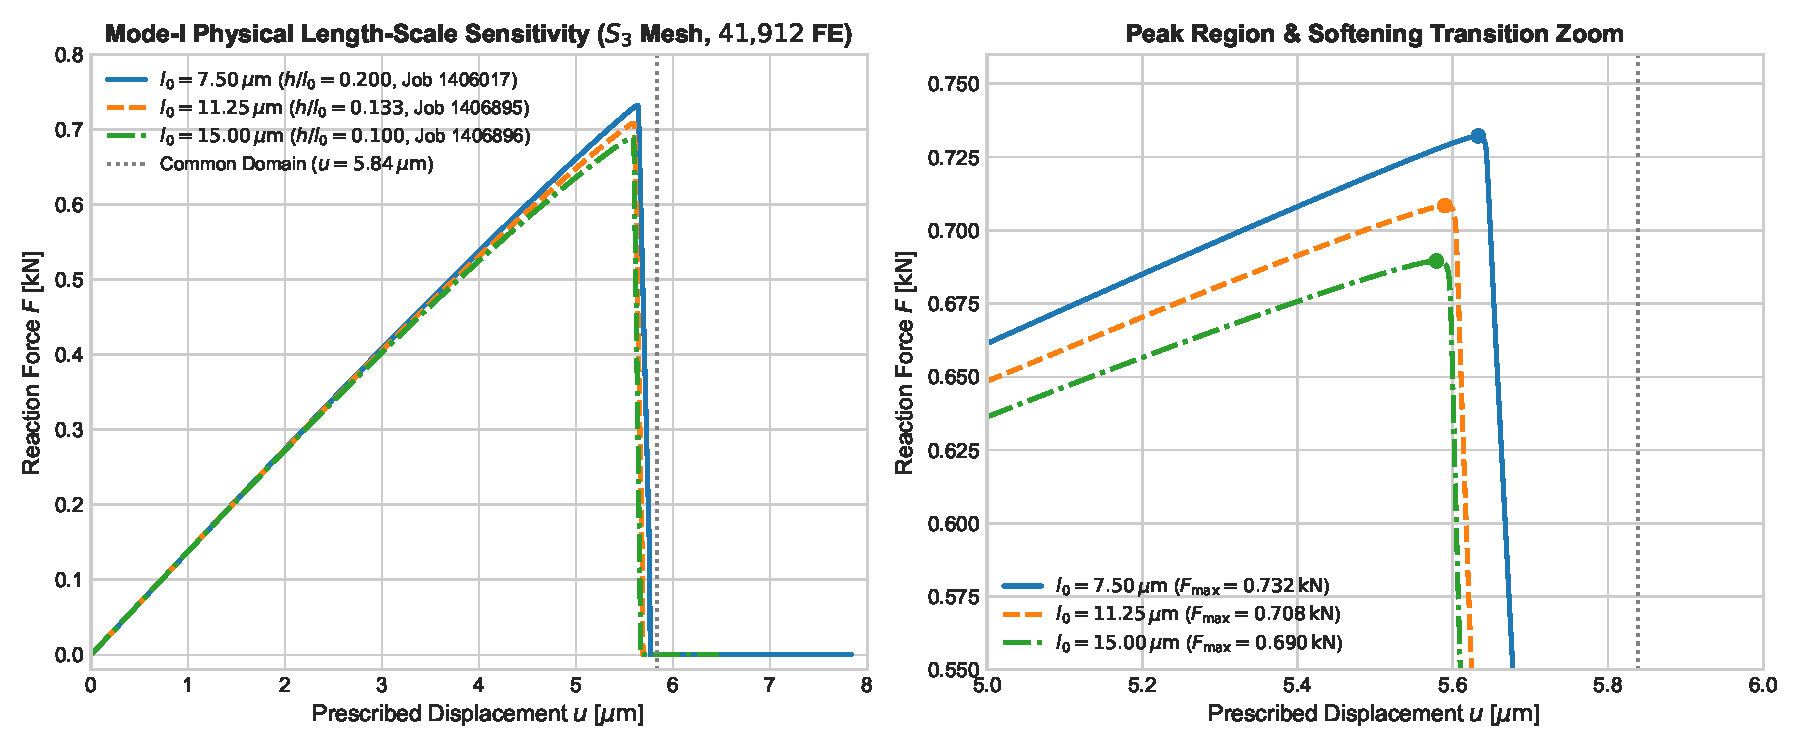
\includegraphics[width=0.88\textwidth]{fig_mode1_clean_l0_sensitivity_fu.pdf}
\caption[Force-displacement response across clean $l_0$ sensitivity sweep.]{Mode-I clean single-variable length-scale ($l_0$) sensitivity on fixed structured $S_3$ mesh ($41{,}912$ FE): (a) global $F$--$u$ response highlighting common comparison domain $u \in [0, 5.839]\,\mu\text{m}$; (b) peak-neighborhood zoom illustrating monotonic load reduction and earlier peak displacement with increasing $l_0$.}
\label{fig:clean_l0_fu_thesis}
\end{figure}

\begin{figure}[htbp]
\centering
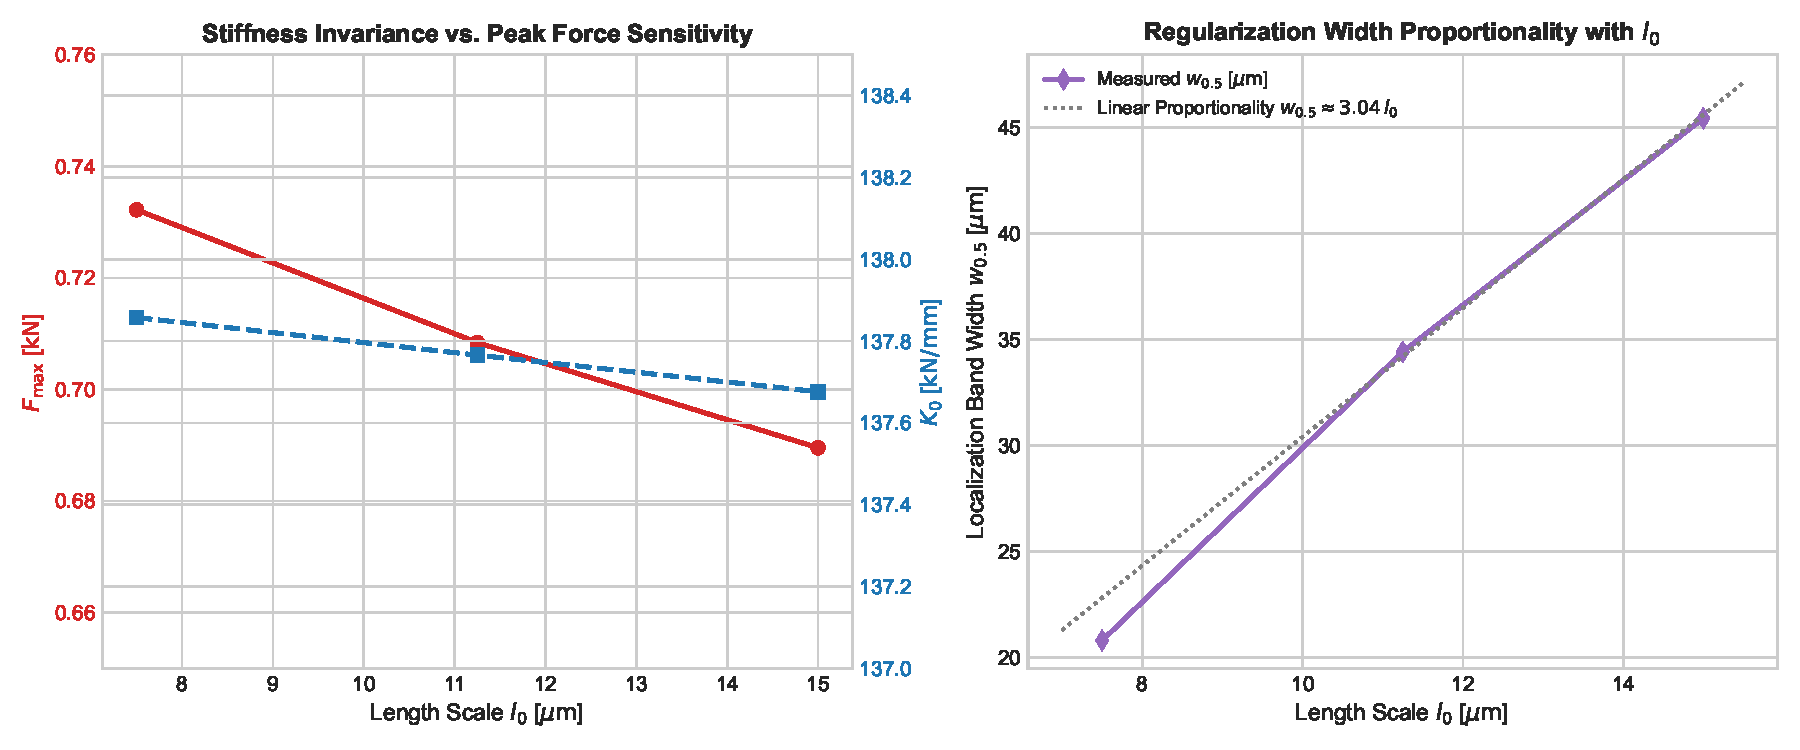
\includegraphics[width=0.92\textwidth]{fig_mode1_clean_l0_scaling_metrics.pdf}
\caption[Scaling metrics across clean $l_0$ sweep.]{Scaling metrics across clean $l_0$ sweep on fixed $S_3$ mesh: (a) initial stiffness $K_0$ invariance; (b) peak reaction force $F_{\max}$; (c) peak displacement $u_{\mathrm{peak}}$; (d) transverse localization profile bandwidth $w_{0.5}$ confirming linear scaling with $l_0$ ($w_{0.5} \approx 3.04\,l_0$).}
\label{fig:clean_l0_scaling_thesis}
\end{figure}

\subsection{Length-Scale Resolution Adequacy for Governed Meshes ($l_0 = 7.5\,\mu\mathrm{m}$)}
\label{sec:length_scale_adequacy_governed_thesis}

To verify that the entire suite of governed production and candidate meshes provides adequate spatial resolution for the phase-field regularisation length scale $l_0 = 7.5\,\mu\text{m}$, discretization metrics were evaluated directly from verified input decks across all six governed models (Table~\ref{tab:governed_mesh_adequacy_thesis}). Sizing is characterized by area-equivalent element size $h_{\mathrm{area}} = \sqrt{A_e}$, notch-root size $h_{\mathrm{notch}}$, and median corridor size $h_{\mathrm{area},\mathrm{med}}$ ($\Omega_{\mathrm{corridor}} = [0.48, 1.02] \times [0.40, 0.60]\,\mathrm{mm}$).

\begin{table}[htbp]
\centering
\caption{Length-scale resolution adequacy metrics for governed Mode-I meshes ($l_0 = 7.5\,\mu\mathrm{m}$). Pure continuum FE mesh nodes are reported; total input deck nodes include $+1$ auxiliary Reference Point (RP) Node \texttt{999999}.}
\label{tab:governed_mesh_adequacy_thesis}
\small
\begin{tabular}{lrrrrrrrr}
\toprule
\textbf{Mesh Configuration} & \textbf{Elements} & \textbf{FE Nodes} & \multicolumn{3}{c}{\textbf{Corridor Sizing [$\mu\mathrm{m}$]}} & \multicolumn{2}{c}{\textbf{Resolution Ratio}} & \textbf{Adequacy Status} \\
\cmidrule(lr){4-6} \cmidrule(lr){7-8}
 & & & $h_{\mathrm{area},\min}$ & $h_{\mathrm{area},\mathrm{med}}$ & $h_{\mathrm{notch}}$ & $\frac{h_{\mathrm{area},\min}}{l_0}$ & $\frac{h_{\mathrm{notch}}}{l_0}$ & \\
\midrule
Fixed Reference ($S_1$) & $15{,}192$ & $15{,}521$ & $2.899$ & $2.931$ & $2.899$ & $\mathbf{0.387}$ & $\mathbf{0.387}$ & \texttt{ADEQUACY\_SUPPORTED} \\
Adaptive ET1 (14k) & $14{,}483$ & $14{,}456$ & $0.760$ & $2.068$ & $1.988$ & $\mathbf{0.101}$ & $\mathbf{0.265}$ & \texttt{ADEQUACY\_SUPPORTED} \\
Adaptive ET2 (6k) & $6{,}112$ & $6{,}181$ & $0.956$ & $4.016$ & $2.632$ & $\mathbf{0.127}$ & $\mathbf{0.351}$ & \texttt{ADEQUACY\_SUPPORTED} \\
Adaptive ET3 (5k) & $5{,}189$ & $5{,}262$ & $1.339$ & $4.898$ & $2.769$ & $\mathbf{0.179}$ & $\mathbf{0.369}$ & \texttt{ADEQUACY\_SUPPORTED} \\
Adaptive ET5 (4k) & $4{,}692$ & $4{,}759$ & $1.230$ & $5.907$ & $3.109$ & $\mathbf{0.164}$ & $\mathbf{0.415}$ & \texttt{ADEQUACY\_SUPPORTED} \\
Spatial Fine (58k) & $57{,}929$ & $57{,}491$ & $0.553$ & $1.947$ & $1.896$ & $\mathbf{0.074}$ & $\mathbf{0.253}$ & \texttt{ADEQUACY\_SUPPORTED} \\
\bottomrule
\end{tabular}
\end{table}

Every governed mesh satisfies the standard phase-field resolution condition ($h/l_0 \le 0.50$) along the fracture path, ensuring that at least $5.2$ elements ($S_1$) up to $27.1$ elements ($58\mathrm{k}$) resolve the core damage zone width ($2 l_0 = 15\,\mu\mathrm{m}$), with notch-root resolution ratio $h_{\mathrm{notch}}/l_0 \le 0.415$ across all configurations.

\section{Spatial Phase-Field Localization, Crack Symmetry, and Bandwidth}
\label{sec:phase_field_contours_and_symmetry}

Figure~\ref{fig:matched_contours_thesis} depicts the full two-dimensional damage field $d(\mathbf{x})$ across crack initiation, limit load, and post-peak extension states.
\begin{itemize}
    \item \textbf{Crack Centroid Path $y_c(x)$}: The damage-weighted centroid offset $|y_c - 0.5\,\text{mm}| \le 3.10\,\mu\text{m}$ across all fixed and adaptive meshes, confirming pure Mode-I horizontal symmetry within discrete element bounds (\textbf{\texttt{CONVERGED / STABLE}}, Figure~\ref{fig:path_dev_thesis}(a)).
    \item \textbf{Diffusive Localization Band Width}: The moderate damage band ($d \ge 0.50$) spans a transverse full-width of $20.0$--$30.0\,\mu\text{m}$ across the ligament ($20.0$--$22.9\,\mu\text{m}$ at $x = 0.55\,\text{mm}$), classified as \textbf{\texttt{MESH-SENSITIVE / RESOLUTION-LIMITED}} (Figure~\ref{fig:ligament_thesis} and Figure~\ref{fig:path_dev_thesis}(b)).
\end{itemize}

\subsection{Baseline Spatial Phase-Field and Crack-Path Comparison: Fixed Reference versus ET1 Adaptive Mesh}
\label{sec:baseline_spatial_ref_vs_et1_thesis}

To establish the baseline spatial convergence foundation of the error-indicator refined configuration, a point-by-point spatial comparison was executed between the qualified fixed-mesh reference ($15{,}192$ finite elements, Job \texttt{1409734.mmaster02}) and the canonical corrected ET1 adaptive baseline ($14{,}483$ finite elements, Package~25, Job \texttt{1409982.mmaster02}). The minimum element size in the adaptive mesh is explicitly disambiguated: $h_{\mathrm{area}} = \sqrt{A_{\min}} = 0.7605\,\mu\mathrm{m}$ represents the area-equivalent length of the smallest triangular element, whereas $h_{\mathrm{edge}} \approx 1.09\,\mu\mathrm{m}$ is the nominal notch-root element edge length. The comparison strictly enforces the matched prescribed displacement protocol ($u \in \{1.0, 3.0, 5.0, 5.733, 5.857, 6.0, 6.5, 7.0, 7.889\}\,\mu\mathrm{m}$) with zero forward-filling beyond the actual solver terminal state ($u_{\mathrm{term}} = 7.889\,\mu\mathrm{m}$).

\begin{enumerate}
    \item \textbf{Pre-Peak Damage Localization \& Elastic Parity ($u \le 5.0\,\mu\mathrm{m}$):}
    \begin{itemize}
        \item Initial structural stiffness $K_0$ matches within $\mathbf{-0.0261\%}$ ($137.909558$ vs $137.945520\,\mathrm{kN/mm}$, $R^2 = 0.99999960$).
        \item Maximum phase-field damage $d_{\max}$ matches closely: $d_{\max} = 0.0095$ vs $0.0091$ at $u=1.0\,\mu\mathrm{m}$; $0.0918$ vs $0.0875$ at $u=3.0\,\mu\mathrm{m}$; $0.3181$ vs $0.2981$ at $u=5.0\,\mu\mathrm{m}$.
        \item For all thresholds $\theta \in \{0.50, 0.70, 0.90\}$, crack-tip position remains stationary at the initial notch root ($x_{\mathrm{tip}} = 0.500000\,\mathrm{mm}$).
        \item Classified as \textbf{\texttt{SPATIAL\_FIELD\_BASELINE\_AGREEMENT}}.
    \end{itemize}

    \item \textbf{Peak-Neighborhood Offset \& Localization Dynamics ($u \in [5.733, 5.857]\,\mu\mathrm{m}$):}
    \begin{itemize}
        \item The adaptive mesh reaches peak load slightly earlier at $u = 5.733\,\mu\mathrm{m}$ ($F_{\max} = 0.743701\,\mathrm{kN}$) compared to the reference mesh at $u = 5.857\,\mu\mathrm{m}$ ($F_{\max} = 0.757778\,\mathrm{kN}$, a $-1.8576\%$ load difference).
        \item At $u=5.857\,\mu\mathrm{m}$, the fixed reference is at peak load with diffuse damage ($d_{\max} = 0.629736, x_{\mathrm{tip}}^{0.90} = 0.500000\,\mathrm{mm}$), whereas the adaptive mesh has already undergone catastrophic snap-through ($d_{\max} = 1.000494, x_{\mathrm{tip}}^{0.90} = 0.976737\,\mathrm{mm}$).
        \item Classified as \textbf{\texttt{SPATIAL\_FIELD\_BASELINE\_DIFFERENCE}}. The earlier adaptive localization and peak shift correlate with differences in local mesh resolution and phase-field evolution; causation is not isolated by the present comparison.
    \end{itemize}

    \item \textbf{Post-Peak Crack Traversal \& Symmetry ($u \ge 6.0\,\mu\mathrm{m}$):}
    \begin{itemize}
        \item Both discretizations achieve full ligament traversal ($x_{\mathrm{tip}}^{0.90} = 0.998490\,\mathrm{mm}$ vs $0.998496\,\mathrm{mm}$, matching the right boundary).
        \item Crack-centroid off-axis deviation $|y_c - 0.500000\,\mathrm{mm}|$ is bounded to sub-micron precision: $\Delta y_{\mathrm{off}} \le 0.461\,\mu\mathrm{m}$ (Reference) and $\Delta y_{\mathrm{off}} \le 0.175\,\mu\mathrm{m}$ (Adaptive ET1).
        \item Transverse localization width matches theoretical $\mathrm{FWHM} = 2 l_0 \ln 2 \approx 20.79\,\mu\mathrm{m}$ across both models.
        \item \textbf{Distinction Between Spatial and Mechanical Discrepancies:} While the spatial crack trajectory and symmetry remain in excellent alignment throughout the post-peak propagation, the reaction force in the fully severed ligament drops below $0.002\,\mathrm{kN}$. Consequently, relative percentage differences between fixed and adaptive models at $u > 6.5\,\mu\mathrm{m}$ are magnified by near-zero division, whereas the absolute reaction force difference is physically negligible ($\Delta F < 0.0015\,\mathrm{kN}$, $<0.25\%$ of peak load).
        \item Classified as \textbf{\texttt{SPATIAL\_FIELD\_BASELINE\_AGREEMENT}}.
    \end{itemize}
\end{enumerate}

\begin{figure}[htbp]
\centering
\includegraphics[width=0.85\textwidth]{gate6_matched_phase_field_contours.png}
\caption[Matched-displacement phase-field damage contours.]{Matched-displacement phase-field damage contours: (top) initiation at $u=5.0\,\mu\text{m}$; (middle) limit load state at $u=5.7\,\mu\text{m}$; (bottom) post-peak propagated crack at $u=6.2\,\mu\text{m}$.}
\label{fig:matched_contours_thesis}
\end{figure}

\begin{figure}[htbp]
\centering
\includegraphics[width=0.78\textwidth]{fig1_fixed_mesh_ligament_profiles.png}
\caption[Ligament phase-field profiles for fixed meshes.]{Ligament phase-field profiles $d(x, y=0.5\,\text{mm})$ for fixed meshes at matched displacement increments.}
\label{fig:ligament_thesis}
\end{figure}

\begin{figure}[htbp]
\centering
\includegraphics[width=0.78\textwidth]{fig4_vertical_path_localization_deviation.png}
\caption[Separation of crack-centroid trajectory and damage localization band width.]{Rigorous separation of (a) crack-centroid trajectory ($|y_c - 0.5| \le 3.1\,\mu\text{m}$, symmetric) and (b) damage localization-band half-width ($10$--$15\,\mu\text{m}$, resolution-limited).}
\label{fig:path_dev_thesis}
\end{figure}

\section{UEL Energy Formulation, Single-IP Rule, and Global Energy Balance}
\label{sec:uel_energy_audit}

\subsection{Implemented Discrete Energy Formulations}
In user subroutine \nolinkurl{f42_mixed_uel.for}, stored elastic strain energy $E_{\mathrm{elas}}$ and fracture surface energy $E_{\mathrm{frac}}$ are evaluated over the $N_{\mathrm{mesh}}$ cells:
\begin{align}
\label{eq:uel_elas_energy}
E_{\mathrm{elas}} &= \sum_{e=1}^{N_{\mathrm{mesh}}} \int_{\Omega_e} \frac{1}{2} g(\bar{d}_e)\,\boldsymbol{\varepsilon} : \mathbb{C}_0 : \boldsymbol{\varepsilon} \,\mathrm{d}\Omega, \\
\label{eq:uel_frac_energy}
E_{\mathrm{frac}} &= \sum_{e=1}^{N_{\mathrm{mesh}}} \int_{\Omega_e} G_c \left[ \frac{\bar{d}_e^2}{2 l_0} + \frac{l_0}{2} |\nabla d|^2 \right] \mathrm{d}\Omega,
\end{align}
where $g(\bar{d}_e) = (1-\bar{d}_e)^2 + k_{\mathrm{res}}$ ($k_{\mathrm{res}} = 10^{-7}$). In the Fortran subroutine implementation, the 2D Gauss integration measure has area dimension $\mathrm{mm^2}$ ($\mathtt{CJAC} = \det(\mathbf{J})\,w$). Under the 2D plane-strain assumption with an implicit unit out-of-plane thickness $B = 1.0\,\mathrm{mm}$, the direct source-algebra units of these whole-element scalar energies are $\mathrm{kN\cdot mm} = \mathrm{J}$. In reporting and tabular presentations, these values are converted to millijoules ($\mathrm{mJ}$) by multiplying by $1000$ exactly once ($1\,\mathrm{kN\cdot mm} = 1\,\mathrm{J} = 1000\,\mathrm{mJ}$). The companion state variables $\mathrm{STATEV}(19)$ and $\mathrm{STATEV}(20)$ evaluate the element area-normalized quotients $\bar{\psi}_f = E_{\mathrm{frac}}^{(e)} / A_e$ and $\bar{\psi}_e = E_{\mathrm{elas}}^{(e)} / A_e$ with direct source dimension $\mathrm{kN/mm} = \mathrm{J/mm^2}$, which are interpretable as volumetric energy densities ($\mathrm{kN/mm^2} = 1\,\mathrm{J/mm^3} = 1000\,\mathrm{mJ/mm^3}$) only under the explicit $1\text{-}\mathrm{mm}$ implicit-thickness convention. External boundary work is evaluated via the discrete trapezoidal boundary-work estimate:
\begin{equation}
\label{eq:wtrap_discrete}
W_{\mathrm{trap},n} = \sum_{i=1}^{n} \frac{F_i + F_{i-1}}{2}(u_i - u_{i-1}).
\end{equation}

\subsection{Single-IP Deduplication Rule}
In the three-layer architecture, companion visualizer elements (Layer 3, CPE4) receive whole-element scalar energies into state variables $\mathrm{STATEV}(17) = E_{\mathrm{frac}}^{(e)}$ and $\mathrm{STATEV}(18) = E_{\mathrm{elas}}^{(e)}$ (in native $\mathrm{kN\cdot mm} = \mathrm{J}$) replicated across all 4 Gauss integration points. Summing across all Gauss points creates a $4\times$ overcounting artifact. Post-processors strictly enforce extraction at \textbf{Integration Point 1 (\texttt{IP1}) only}, recovering the once-per-underlying-finite-element global energy sum under the 2D implicit-unit-thickness convention.

\subsection{Non-Invasiveness and Mechanical Parity Verification}
Energy logging is mathematically decoupled from the element residual vector (\texttt{RHS}) and stiffness matrix (\texttt{AMATRX}). Controlled HPC benchmarks established:
\begin{center}
  \textbf{\texttt{ENERGY\_SOURCE\_MECHANICAL\_PARITY --- QUALIFIED (COMMON QUAD FORMULATION)}}
\end{center}
Global mechanical force trajectories were identical ($|\Delta F| = 0.0\,\text{kN}$) against uninstrumented baselines across:
\begin{itemize}
    \item \textbf{Elastic Parity (Job 1406904 vs 1406905, 30 incs)}: Exact force trajectory agreement ($|\Delta F| = 0.00000000\,\text{kN}$).
    \item \textbf{Full Softening Parity (Job 1406906 vs 1406907, 129 incs)}: Exact force trajectory agreement through complete failure to $u = 0.035\,\text{mm}$ ($|\Delta F| = 0.0\,\text{kN}$, $d_{\max} = 0.977$, $74.2\%$ softening drop).
\end{itemize}
Old-run $d/\mathcal{H}$ state-field parity was not observable in standard ODBs and triangle parity was not established.

\subsection{Discrete Potential Disproval and Observability Boundary}
Because the staggered solver alternates between displacement $\mathbf{u}_n$ and phase field $d_{n+1}$, discrete cross-derivatives do not commute:
\begin{equation}
\label{eq:cross_derivative_incompatibility}
\frac{\partial^2 \Pi}{\partial \mathbf{q}_u\,\partial \mathbf{q}_d} \ne \frac{\partial^2 \Pi}{\partial \mathbf{q}_d\,\partial \mathbf{q}_u}.
\end{equation}
Consequently, \textbf{\texttt{COMMON\_DISCRETE\_POTENTIAL\_DISPROVEN\_BY\_CROSS\_DERIVATIVE\_INCOMPATIBILITY}} governs. The two-term bookkeeping difference is defined as:
\begin{equation}
\label{eq:bookkeeping_diff_def}
\text{TWO\_TERM\_BOOKKEEPING\_DIFFERENCE}(u) \equiv W_{\mathrm{trap}}(u) - \left[ E_{\mathrm{elas}}(u) + E_{\mathrm{frac}}(u) \right].
\end{equation}
Because standard Abaqus ODB files do not persist within-increment Newton paths, \textbf{\texttt{DECOMPOSITION\_REQUIRES\_WITHIN\_INCREMENT\_PATH\_INFORMATION}} applies, and \textbf{\texttt{GLOBAL\_ENERGY\_IDENTITY --- NOT\_YET\_CLOSED}} is strictly maintained.

\begin{figure}[htbp]
\centering
\includegraphics[width=0.80\textwidth]{fig_mode1_s1_energy_balance.pdf}
\caption[Global energy evolution for baseline $S_1$.]{Global energy component evolution for the baseline $S_1$/$T_2$ trajectory ($15{,}192$ elements). The two-term bookkeeping difference remains within $\pm0.008\%$ over the specifically qualified pre-peak $S_1$/$T_1$--$T_3$ trajectories. In the post-peak regime it reaches $+0.7607\%$ for $S_1$/$T_2$. This quantity is an endpoint bookkeeping difference and is not interpreted as an energy residual or conservation error. \textbf{\texttt{GLOBAL\_ENERGY\_IDENTITY --- NOT\_YET\_CLOSED}}.}
\label{fig:energy_balance_thesis}
\end{figure}

\begin{table}[htbp]
\centering
\caption{Global energy bookkeeping audit for completed uniform mesh cases ($u = 0.010\,\text{mm}$).}
\label{tab:energy_audit_thesis}
\small
\begin{tabular}{lrrrr}
\toprule
\textbf{Energetic Quantity} & \textbf{Case $T_1$ (Coarse $\Delta t$)} & \textbf{Case $T_2$ (Nominal $\Delta t$)} & \textbf{Case $T_3$ (Fine $\Delta t$)} & \textbf{Case $S_1$ (Baseline)} \\
\midrule
Boundary Work $W_{\mathrm{trap}}$ [$\text{mJ}$] & $2.41011$ & $2.35933$ & $2.33189$ & $2.35933$ \\
Elastic Energy $E_{\mathrm{elas}}$ [$\text{mJ}$] & $0.00104$ & $0.00116$ & $0.00120$ & $0.00116$ \\
Fracture Energy $E_{\mathrm{frac}}$ [$\text{mJ}$] & $2.39995$ & $2.34022$ & $2.24813$ & $2.34022$ \\
Bookkeeping Diff [$\text{mJ}$] & $0.00912$ & $0.01795$ & $0.08256$ & $0.01795$ \\
Normalized Difference & $\mathbf{0.3783\,\%}$ & $\mathbf{0.7607\,\%}$ & $\mathbf{3.5408\,\%}$ & $\mathbf{0.7607\,\%}$ \\
\bottomrule
\end{tabular}
\end{table}
